\documentclass[landscape]{article}

\usepackage{tboxen}
\usepackage{url}
\usepackage{amsmath}
\usepackage{amssymb}
\usepackage{epsfig}
\usepackage[tight]{subfigure}
\usepackage{color}
\usepackage{type1cm}
\usepackage{tabularx}
\usepackage{subfig}
\usepackage[none]{hyphenat}

% Custom variables

\newcommand{\argmax}[1]{\underset{#1}{\operatorname{arg}\operatorname{max}}\;}

% How much length we want to add to the poster while editing.  Note
% that these are just integer variables.  There is probably a better
% way to do this...
\newcounter{width}
\newcounter{height}
\newcounter{extra-length}
% these are in cm
\setcounter{width}{110}
\setcounter{height}{68} % developing at 2/3 magnification for 40x65in poster
\setcounter{extra-length}{0} % for development

% Boolean variable: whether or not we want to show grid lines
\newif\ifusegrid
%\usegridtrue
\usegridfalse

% You can define any rgb colors you want for the background.  The
% first two lines define a blue to cream fade.  See how they are used
% below.
\definecolor{bottomcolor}{rgb}{ 0.538, 0.663, .788}
\definecolor{topcolor}{rgb}{    0.538, 0.663, .788}
% Uncomment these next two lines if you want to have an all white background.
%\definecolor{topcolor}{rgb}{1,1,1}
%\definecolor{bottomcolor}{rgb}{1,1,1}

% Other counters that we will use below.
\newcounter{grid-top}
\newcounter{grid-right}
\newcounter{title-top}
\newcounter{title-left-margin}
\newcounter{title-width}
\newcounter{title-left}
\newcounter{title-box-width}

% ==============================================================================
% Set up paper sizes

\newcounter{total-height}
\setcounter{total-height}{\arabic{height} + \arabic{extra-length}}
\setlength{\paperwidth}{\arabic{width}cm}
\setlength{\paperheight}{\arabic{total-height}cm}
\setlength{\textwidth}{\paperwidth}
\setlength{\textheight}{\paperheight}

% These usually stay the same for tboxen
\setlength{\headheight}{0 cm}
\setlength{\headsep}{0 cm}
\setlength{\topmargin}{-2 cm} 
\setlength{\oddsidemargin}{-1in}

% From tboxen:
% this is often necessary for pdf and dvips to work
\ifx\pdfoutput\undefined 
% for dvi
\special{papersize=\arabic{width}cm,\arabic{height}cm}
\else 
% for pdf
\pdfpagewidth=\paperwidth 
\pdfpageheight=\paperheight 
\fi 

% ==============================================================================
% POSTER STARTS HERE
\begin{document}
\begin{center}
  
  % ==============================================================================
  % Main body
  \begin{tikzpicture}
    
    % This defines your background box - entries are pretty self explanatory.
    % The colors ``topcolor'' and ``bottomcolor'' are defined above.
    \shade[top color = topcolor,
      bottom color = bottomcolor,
      rounded corners = 1cm, % The larger this is, the rounder your corners
      line width = 2mm, % The width of your border lines
      draw]
    (0,0) rectangle +(\textwidth-2cm,\textheight-1cm); 
    % This last line above just sets up the bounding box for the whole poster.  You don't want to change it.

    % ==============================================================================
    \ifusegrid
    % Draw grid guidelines if desired.
    \setcounter{grid-top}{\arabic{total-height}-1}
    \setcounter{grid-right}{\arabic{width}-2}
    \draw[style=help lines] (0,\arabic{extra-length}) grid (\arabic{grid-right},\arabic{grid-top});
    \setcounter{grid-top}{\arabic{height}-1}
    \foreach \x in {0,5,...,\arabic{grid-right}}
    \foreach \y in {0,5,...,\arabic{grid-top}}
    \draw (\x,\y) + (0,\arabic{extra-length}) node{\tiny \x,\y};
    \fi

    % ==============================================================================
    % Title box
    %
    % The following defaults make the title box span the whole top,
    % start 3cm from the top, and end 2 cm from both sides. I have
    % hard-coded the 2s and 3 below.  Play around with the trade-off
    % between changing these numbers and changing
    % ``title-left-margin'' if you are not happy with the defaults.
    \setcounter{title-left-margin}{0} % This specifies the additional padding to the right and left of the title.  Can be negative.
    \setcounter{title-top}{\arabic{total-height}-3} % Places the top of the title 3 cm from the top of the poster.
    \setcounter{title-width}{\arabic{width}-2*\arabic{title-left-margin} - 2*2 - 4} % Automatically calculates the width of the title based on the margin.
    \setcounter{title-left}{\arabic{title-left-margin} + 2} % Automatically places the title 2m from the left edge of the poster + the user specified margin.
    \setcounter{title-box-width}{\arabic{width} - 30}
    \path (\arabic{title-left},\arabic{title-top}) node(title) [style=tbox, text width=\arabic{title-width}cm] {
      \begin{center}

        % Three parboxes allow for images on both sides of the title
        % box with the title text in the middle.
        \parbox{10cm} {
        
\includegraphics[height=6cm]{../../figures/berkeley_seal.pdf}
        }
        \parbox{\arabic{title-box-width}cm} {
          \centering
              {\Huge \bf{Timely Object Recognition} } \\
              \vspace{1cm}
              \begin{tabular}{cccc}
                {\Large Sergey Karayev$^1$, \hfill} & {\Large Tobias Baumgartner$^2$, \hfill} & {\Large Mario Fritz$^3$, \hfill} & {\Large Trevor Darrell$^1$}\\\\
                \multicolumn{4}{c}{\large $^1$UC Berkeley, \hspace{2cm} $^2$RWTH Aachen, \hspace{2cm} $^3$MPI Informatics}
              \end{tabular}
        }
        \parbox{10cm} {
          
\includegraphics[width=10cm]{../../figures/MPI_logo.png}
        }

      \end{center}
    };
    
    %%% MOTIVATION
    \path (title.south west) ++(0cm,-2cm) + (-\arabic{title-left-margin}cm,0cm) node(motivation) [style=tbox,text width=28cm] {
    \textbf{\textsc{Problem}}
    \begin{itemize}
      \item Detect objects of many classes in an image.
      \item Trained detectors and classifiers already exist, but there is \textbf{not enough time to run all detectors}.
    \end{itemize}

    \textbf{\textsc{Approach}}
    \begin{itemize}
      \item Formulate \textbf{timeliness} evaluation of detection performance vs. time.
      \item Treat detectors and classifiers as ``black boxes''; use reinforcement learning to find a \textbf{dynamic} policy for deploying them.
    \end{itemize}

    \textbf{\textsc{Results}}
    \begin{itemize}
      \item Learn to take actions that do not provide immediate reward.
      \item Wrapping per-class detectors in our system and setting a deadline\\\textbf{increases the multi-class Average Precision at deadline and before.}
    \end{itemize}
    }; \addcenteredtitle{motivation}{1. Motivation}
    
    %%% MODEL & REINFORCEMENT LEARNING
    \path (motivation.south west) ++(0cm,-2cm) node(implementation) [style=tbox,text width=28cm] {
      \textbf{\textsc{AP vs Time and the Reward Function}}\\
      \parbox{13cm}{
      \begin{itemize}
        \item The final evaluation is the normalized area under the AP vs. Time curve between $T_s$ and $T_d$.
        \item Because this is additive per action, we define \begin{align*} R(s^j,a) = \Delta \text{ap} (t_T^j-\frac{1}{2}\Delta t) \end{align*}
      \end{itemize}
      }
      \parbox{15cm}{\hfill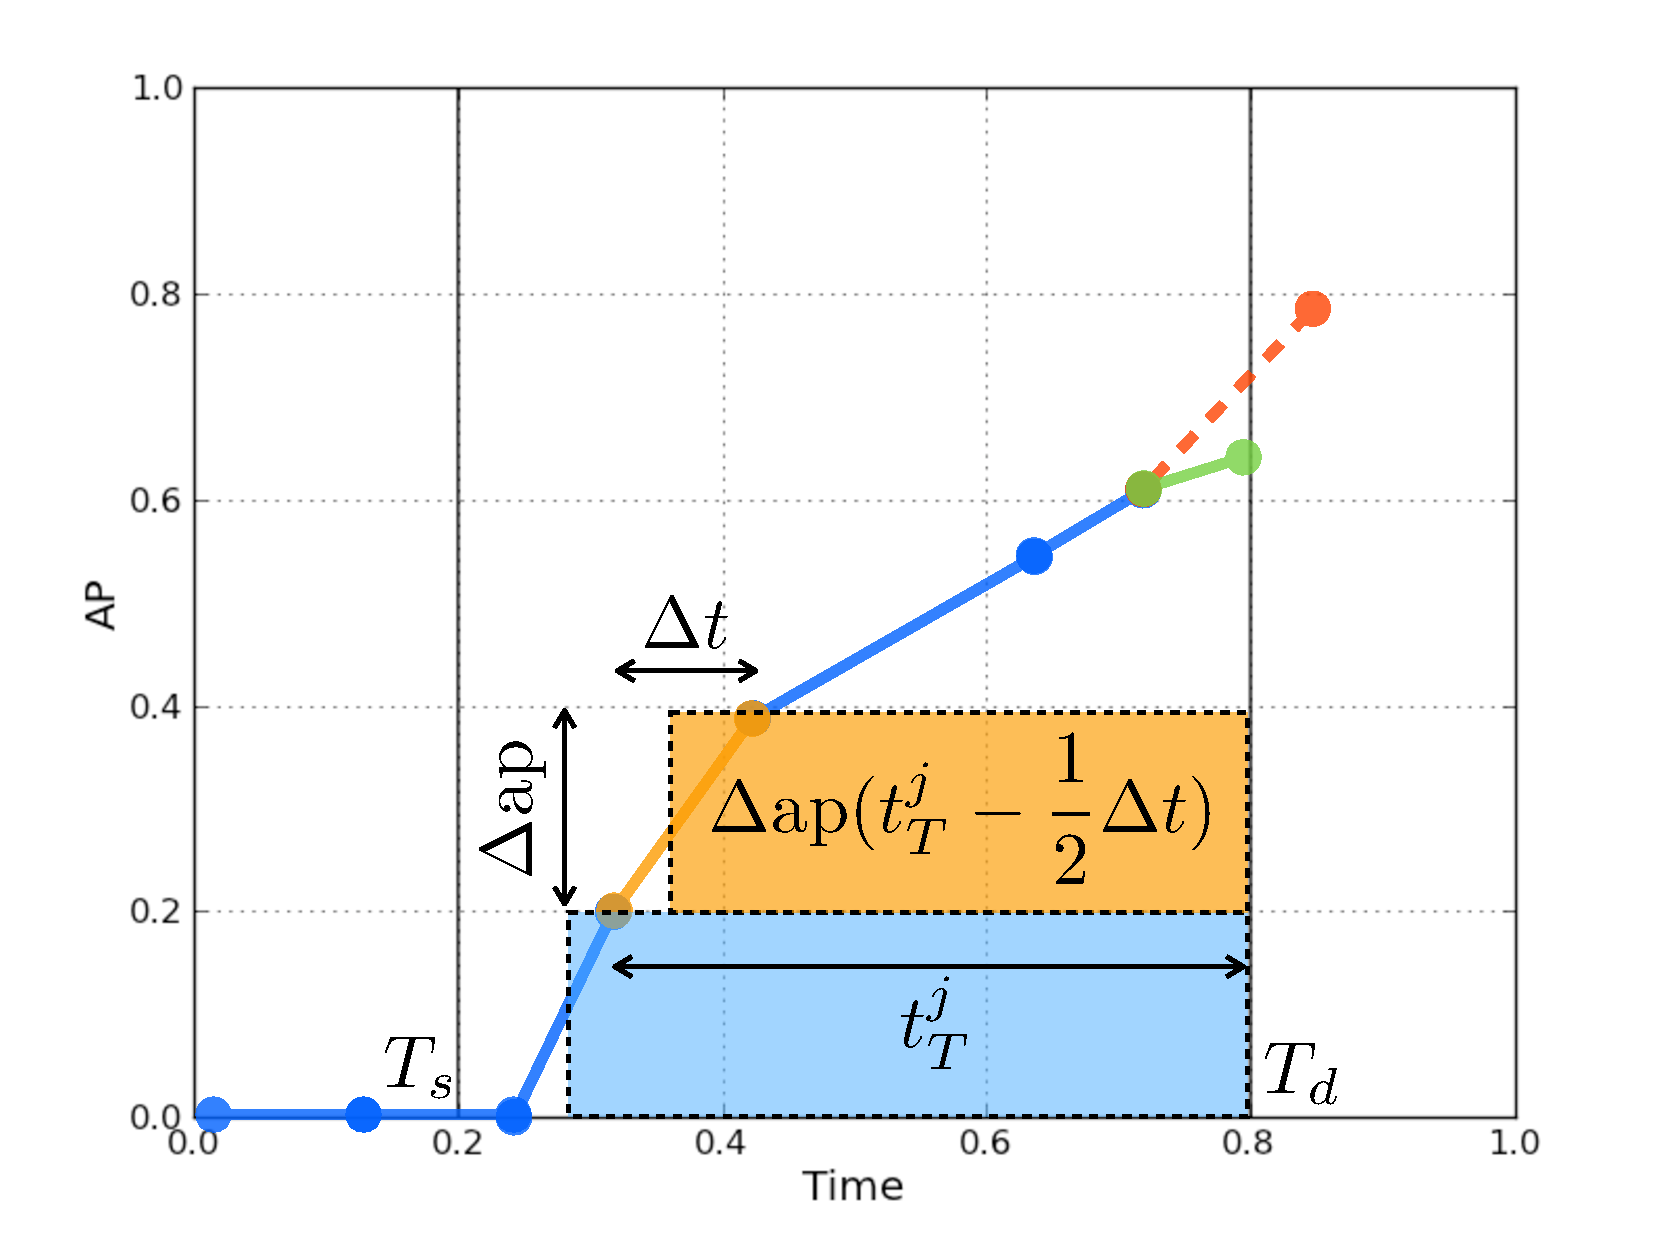
\includegraphics[width=14cm]{../../figures/apvst_expl.pdf}}
      \vspace{7mm}
      
      \textbf{\textsc{Reward discount $\gamma$}}
      \begin{itemize}
      \item $\gamma=0$ induces a completely greedy policy; at $\gamma=1$ is full lookahead.
      \item $\gamma = 0.4$ performs best in cross-validation on the final evaluation.
      \end{itemize}
      \vspace{1cm}

      \textbf{\textsc{Learn $\pi(s)$}} with Monte Carlo policy iteration.
      \begin{itemize}
        \item Gather samples under current $\pi$ by running detection episodes on several thousand images.
        \item Update policy-defining weights $\theta$ with $L_1$ regularization.
        \item Gradually decrease $\epsilon$-greediness of policy.
      \end{itemize}
      \vspace{1cm}

      \textbf{\textsc{The belief state}} posterior over class presences $P(\mathbf{C}|\mathbf{o})$ is updated with observations $\mathbf{o}$.
      \begin{itemize}
        \item \emph{Direct} method assumes independence between classes, and simply replaces the posterior of the class(es) corresponding to the action.
        \item \emph{MRF} method sets evidence node and runs loopy BP in a fully-connected MRF model learned with $L_1$-regularization.
      \end{itemize}
    }; \addcenteredtitle{implementation}{3. Implementation}

    %%% FIGURE 1
    \path (motivation.north east) ++(2cm,0cm) node(figure1) [style=tbox,text width=38cm] {
      \begin{center}
        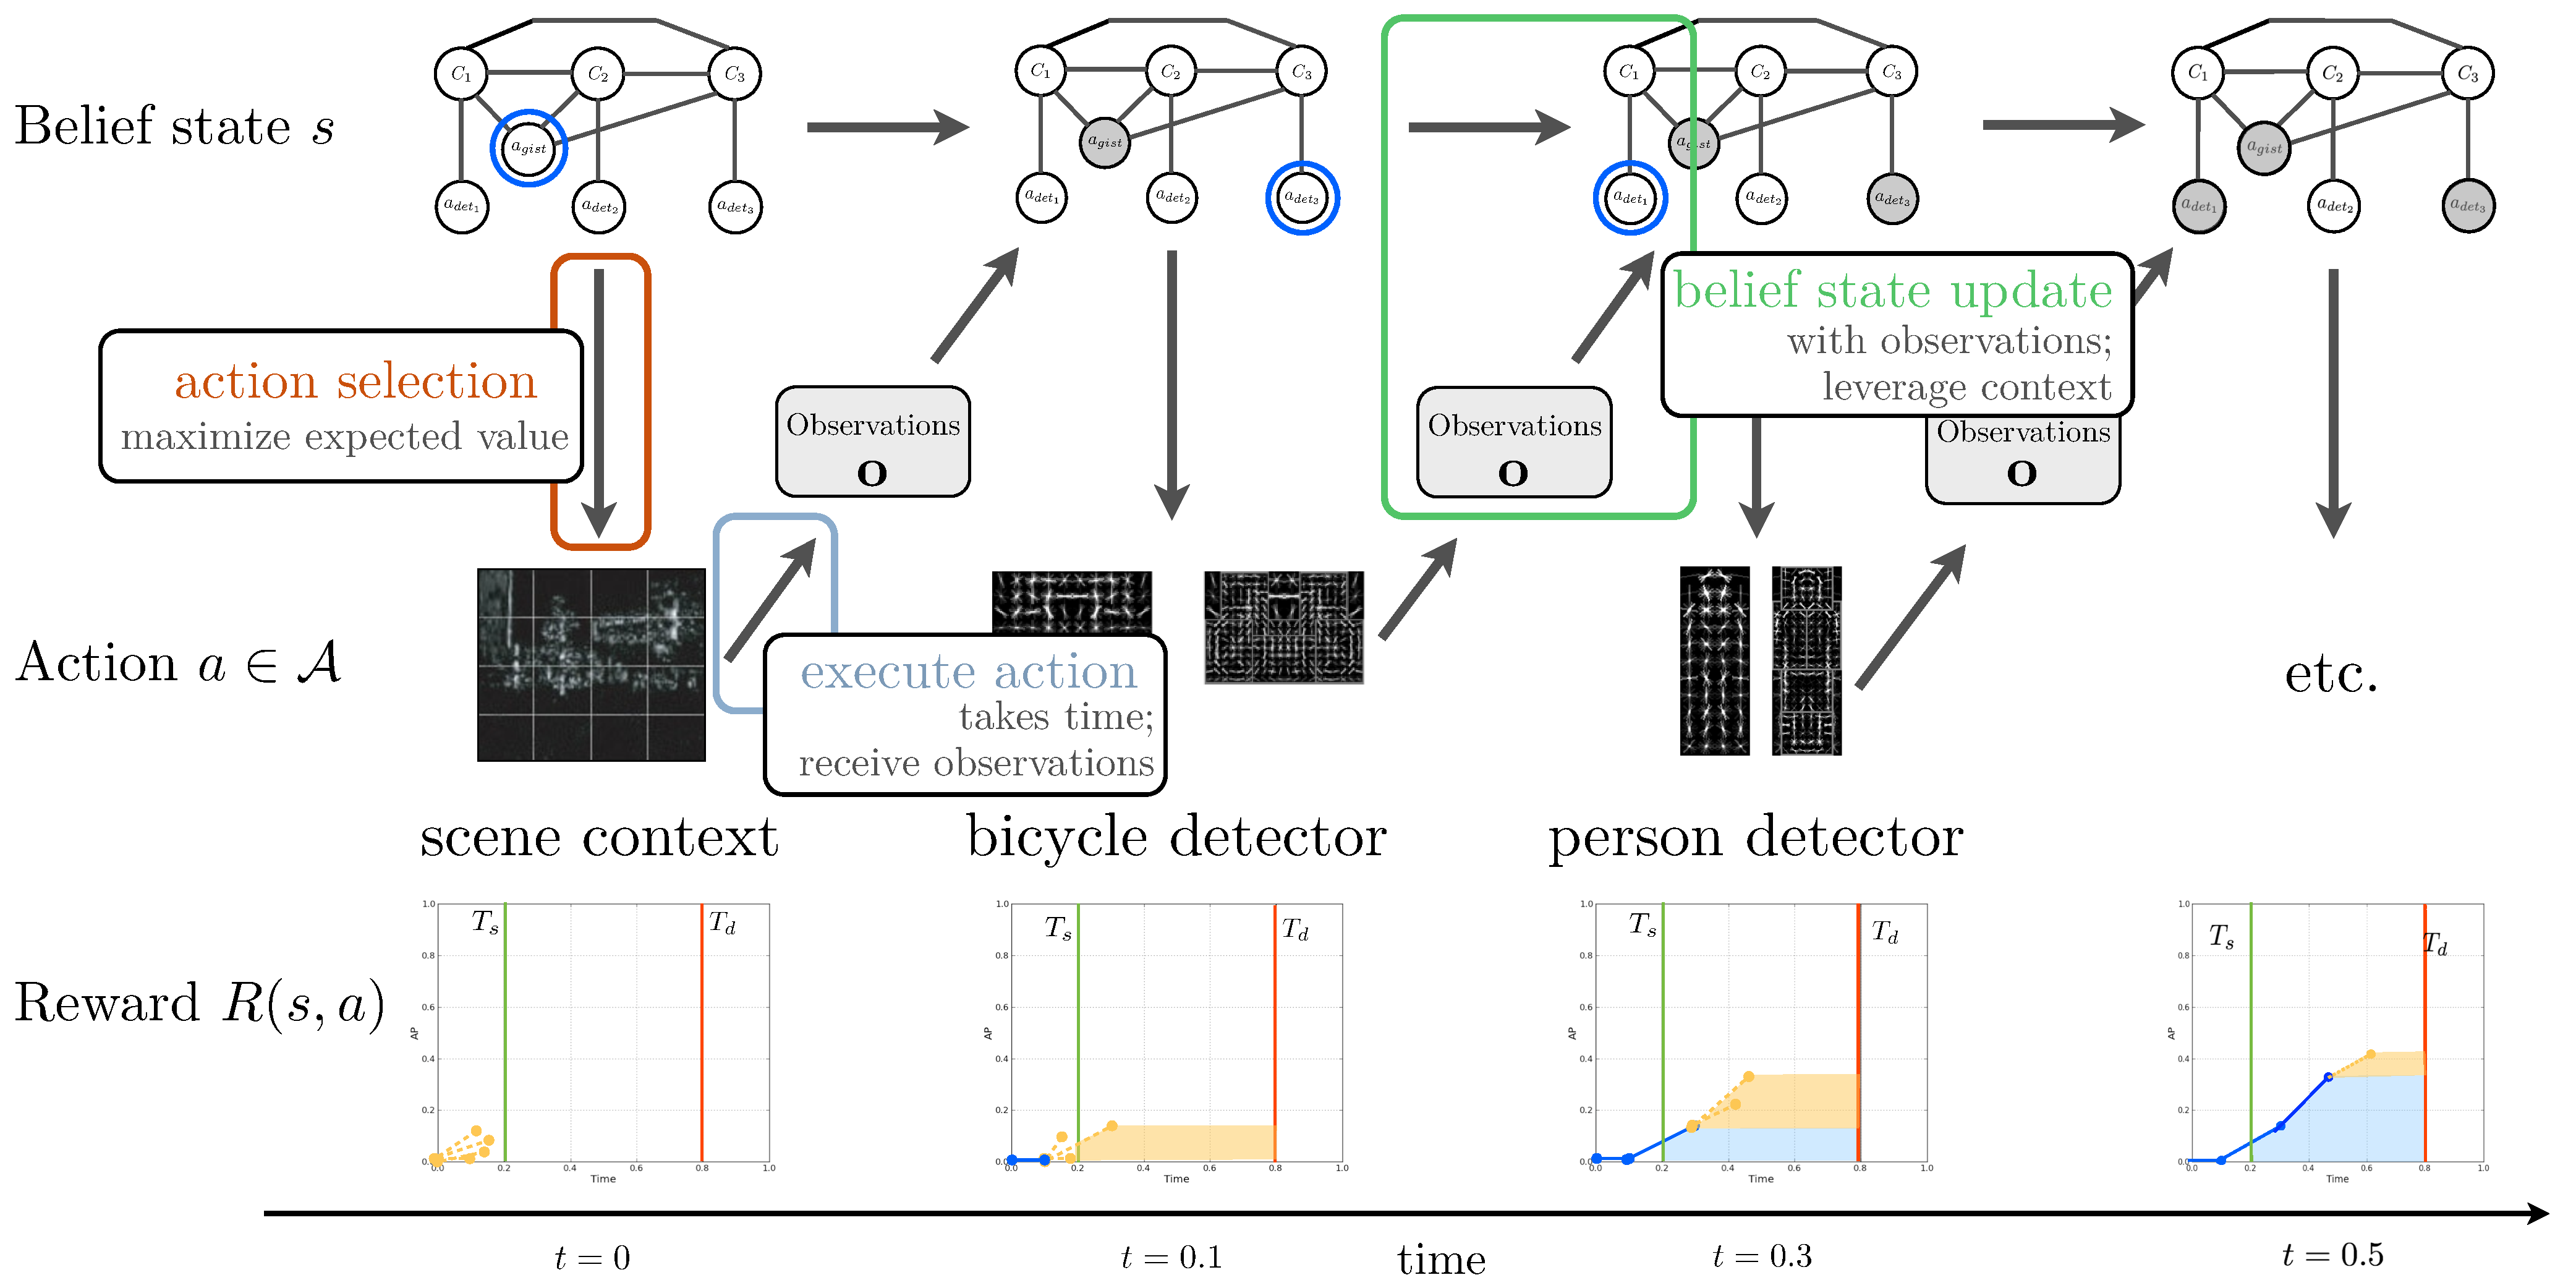
\includegraphics[width=38cm]{../../figures/figure1_with_pomdp.pdf}
      \end{center}
      \begin{itemize}
        \item Action $a \in \mathcal{A}$ can run detector of object class $k$ on whole image, or classify the scene.
        \item The selected action returns observations $\mathbf{o}$: a list of detections, or an evaluated feature.
        \item Define the policy as taking the untaken action with maximum value, linearly approximated: \begin{align*} \pi(s) = \argmax{a \in \mathcal{A} \setminus \mathcal{O}} Q(s,a) = \theta_\pi^\top \phi(s,a) \end{align*}
        \item Learn an accurate approximation to the expected rewards to the end of the episode: \begin{align*}Q^\pi(s^j,a^j) = \mathbb{E} [R \mid s^j, a^j, \pi]\end{align*} where $R = \sum_{i=j}^J \gamma^{i-j} R(s^i,a^i)$ and $J$ is the index of the last action before deadline time $T_d$.
      \end{itemize}
    }; \addcenteredtitle{figure1}{2. Sequential Multi-class Detection}

%%% FEATURES AND WEIGHTS
    \path (figure1.south west) ++(0cm,-2cm) node(features) [style=tbox,text width=38cm] {
      The featurization of the belief state and considered action $\phi(s, a)$ reflects
      \begin{itemize}
        \item current probabilities of presence for all classes, and associated entropies;  
        \item current time to $T_s$ and to $T_d$, and the expected time of the action.
      \end{itemize}
      \vspace{5mm}

      \parbox{18cm}{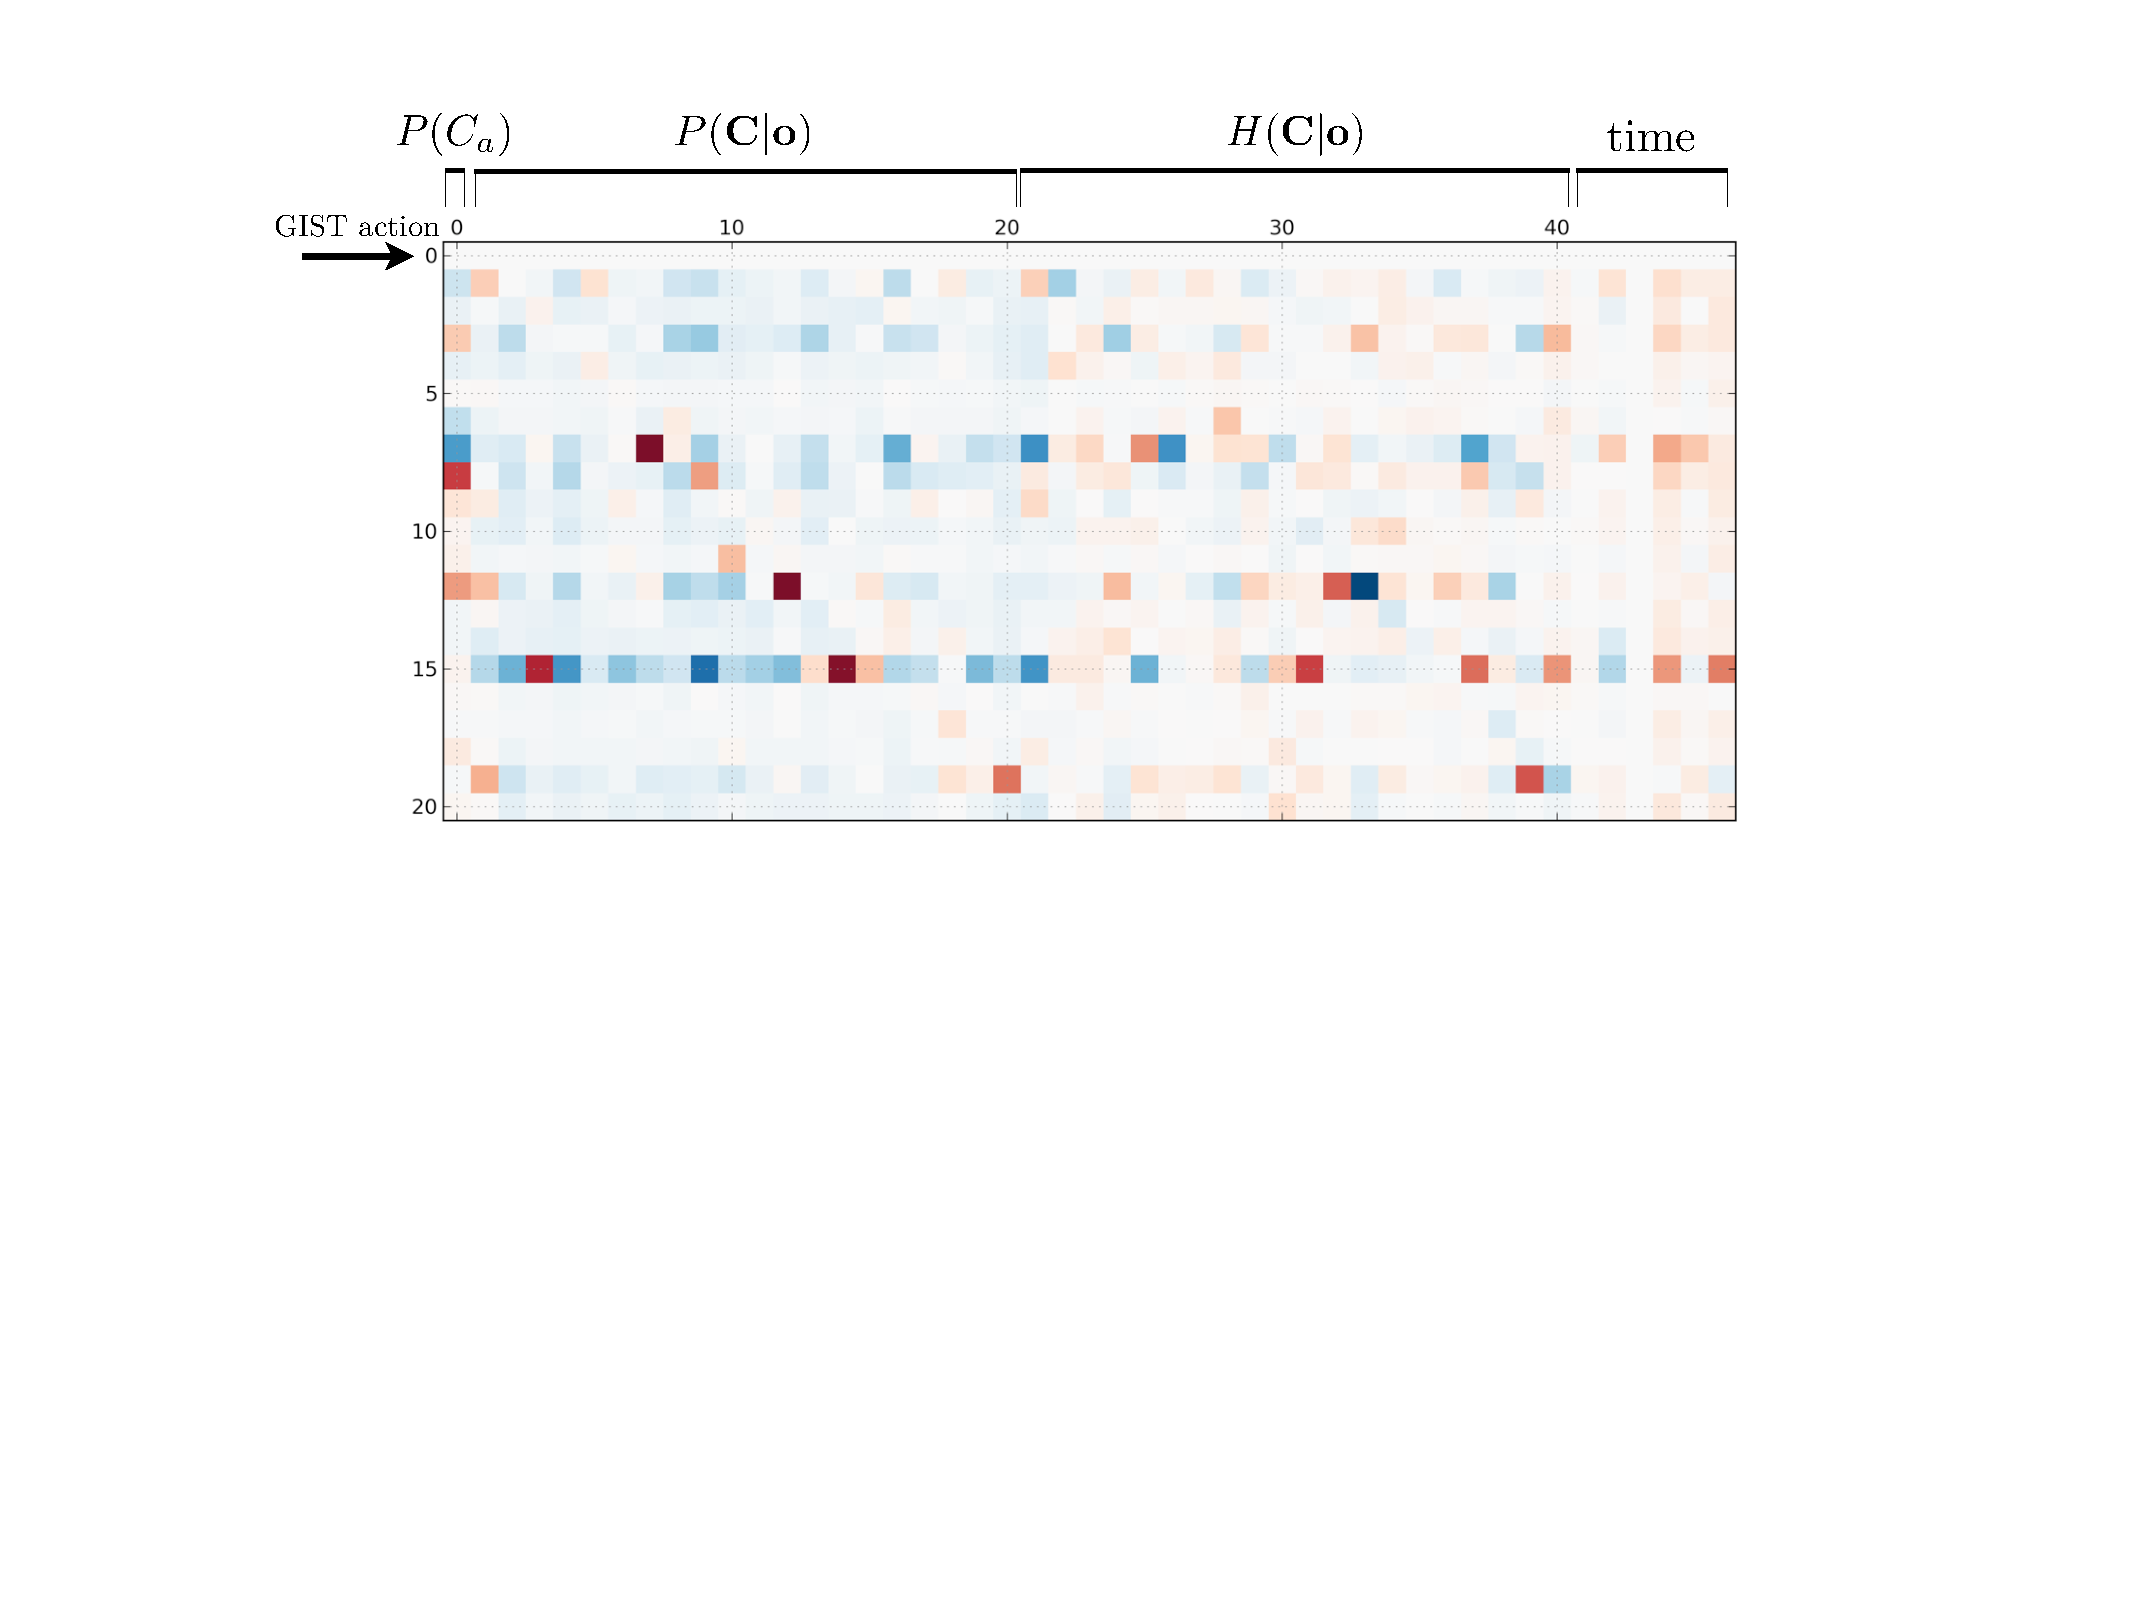
\includegraphics[width=17cm]{../../figures/weights_greedy.pdf}\\\centering \small{\textbf{Greedy}}}\hfill%
      \parbox{18cm}{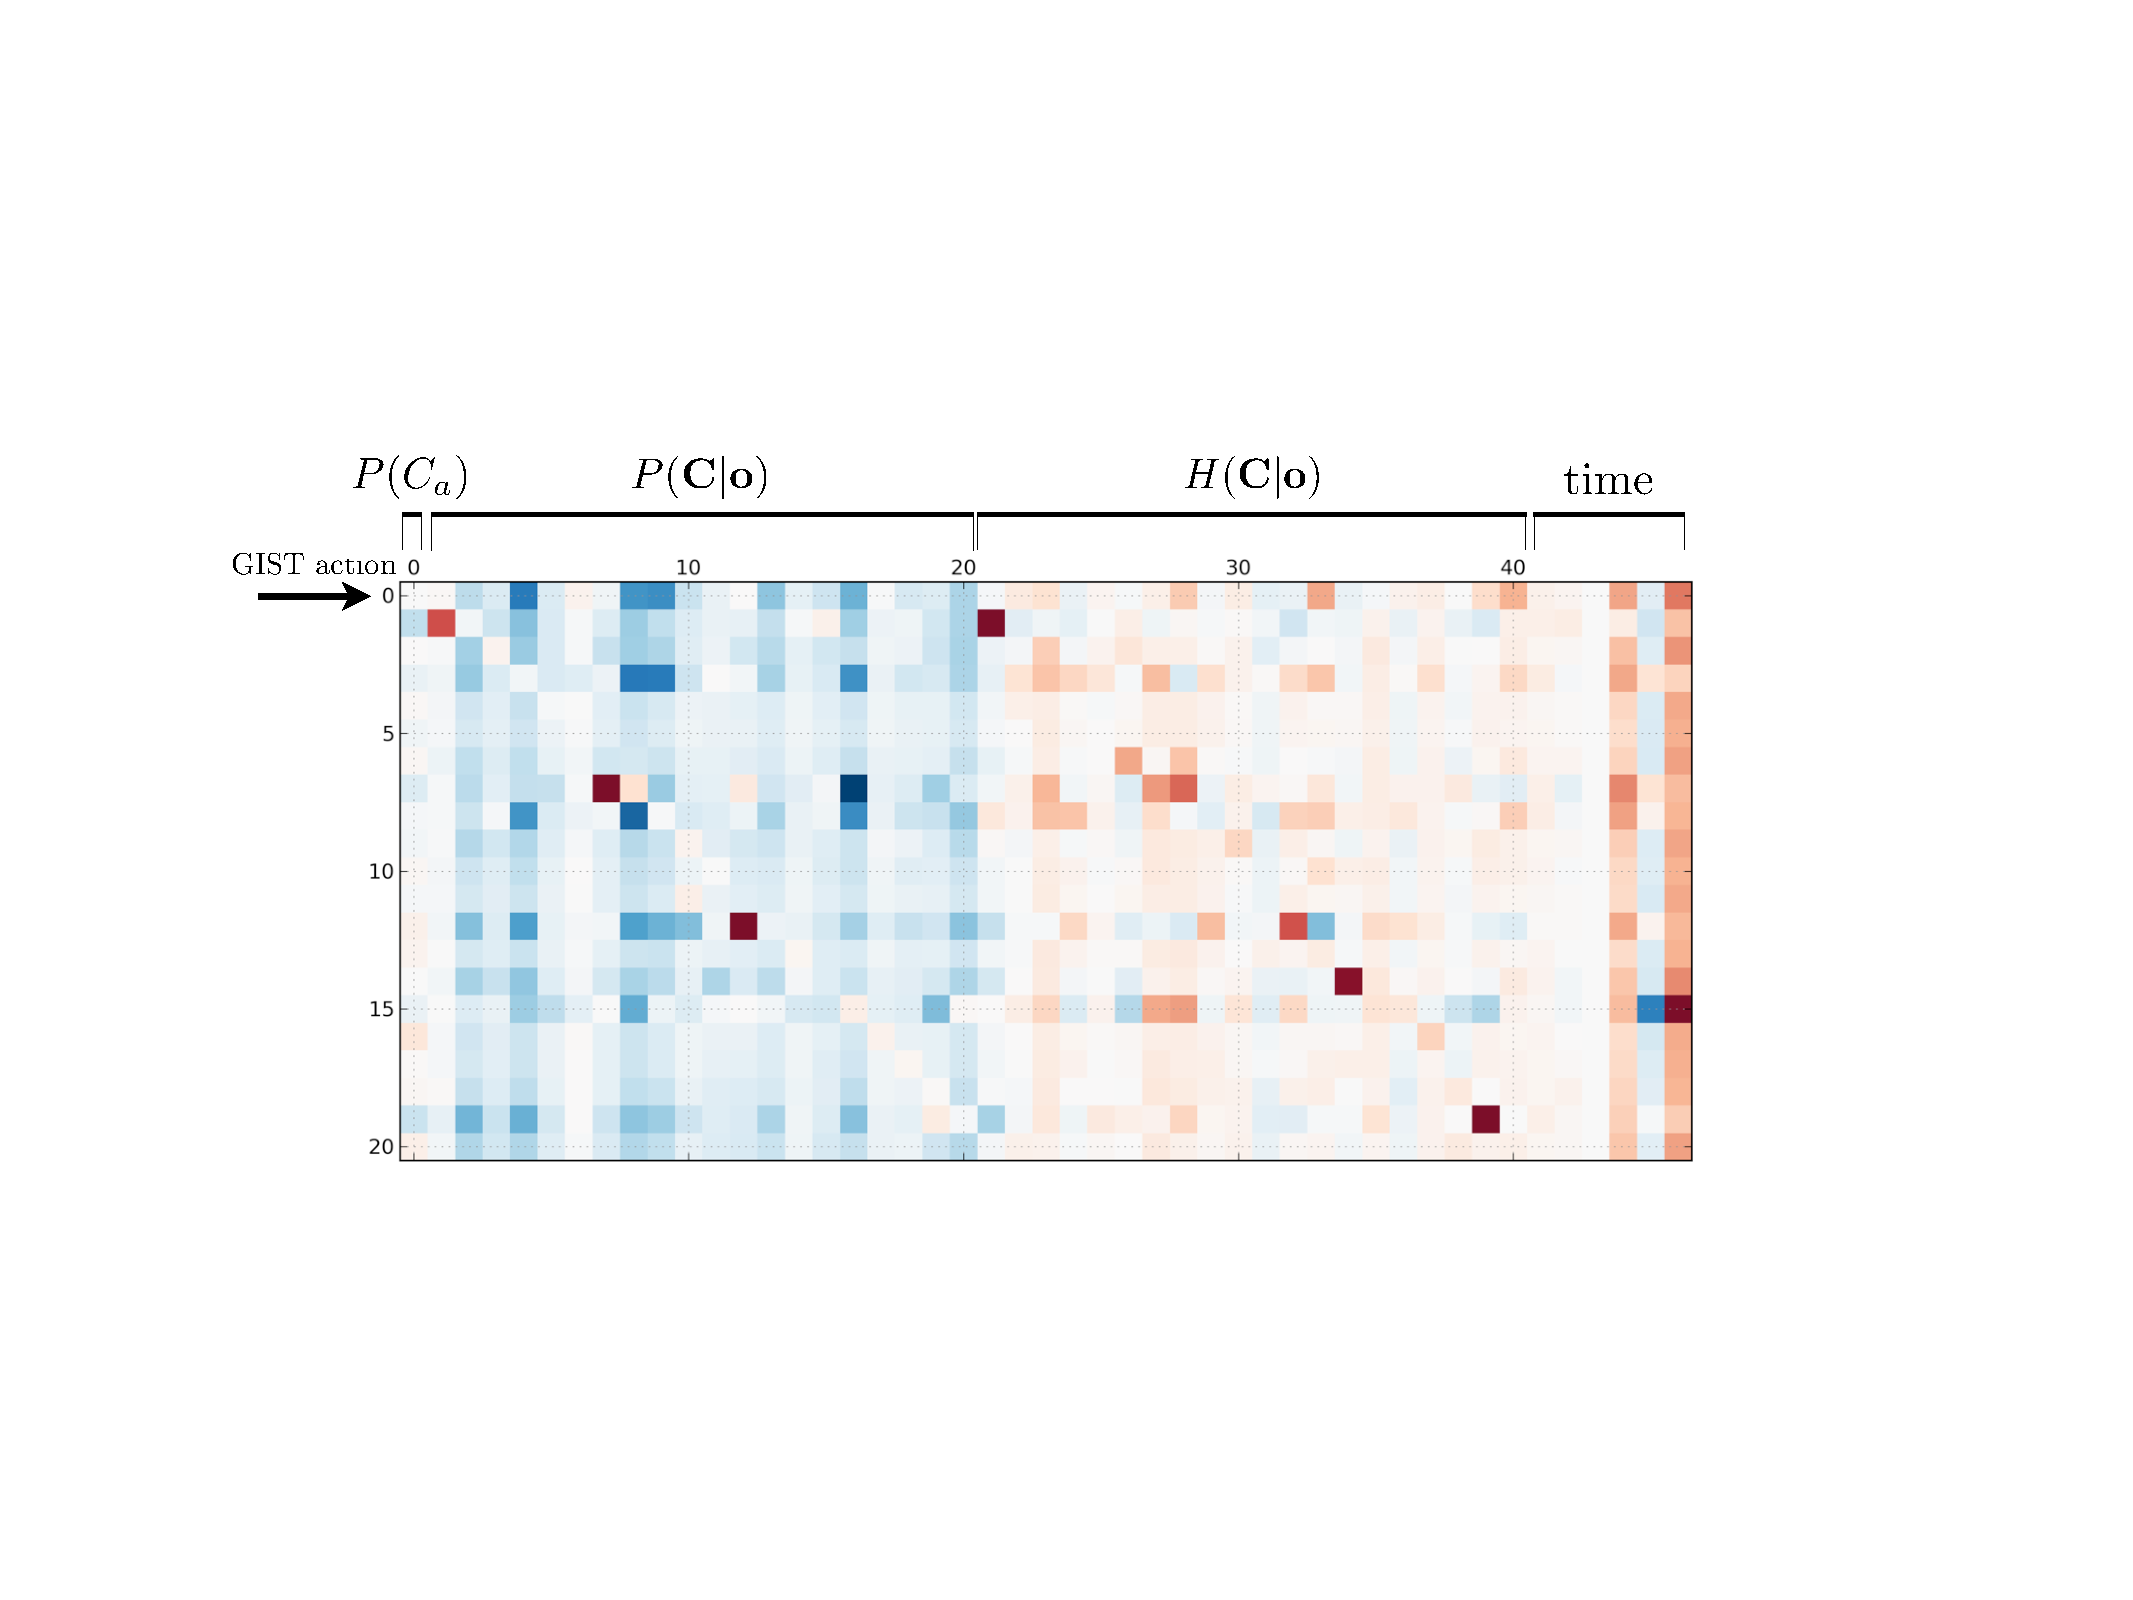
\includegraphics[width=17cm]{../../figures/weights_rl.pdf}\\\centering \small{\textbf{Reinforcement Learning}}}\\
      \begin{center}Learning with a higher $\gamma$ results in policies reliant on the global scene feature.\end{center}
    }; \addcenteredtitle{features}{4. Feature Representation and Policy Weights}

%%% RESULTS
    \path (figure1.north east) ++(2cm,0cm) node(results) [style=tbox,text width=28cm] {
      We evaluated on the PASCAL VOC 2007 detection task, using
      \begin{itemize}
        \item 20 Deformable Part Model detectors (one per class)
        \item a scene context action based on the GIST feature.
      \end{itemize}
      \vspace{5mm}

      \textbf{\textsc{Performance vs. Time}}\\
      \parbox{14cm}{
      Our method is compared to a random, optimal static, and oracle orderings, evaluated at different settings of start and deadline times.
      \vspace{2mm}
      \begin{center}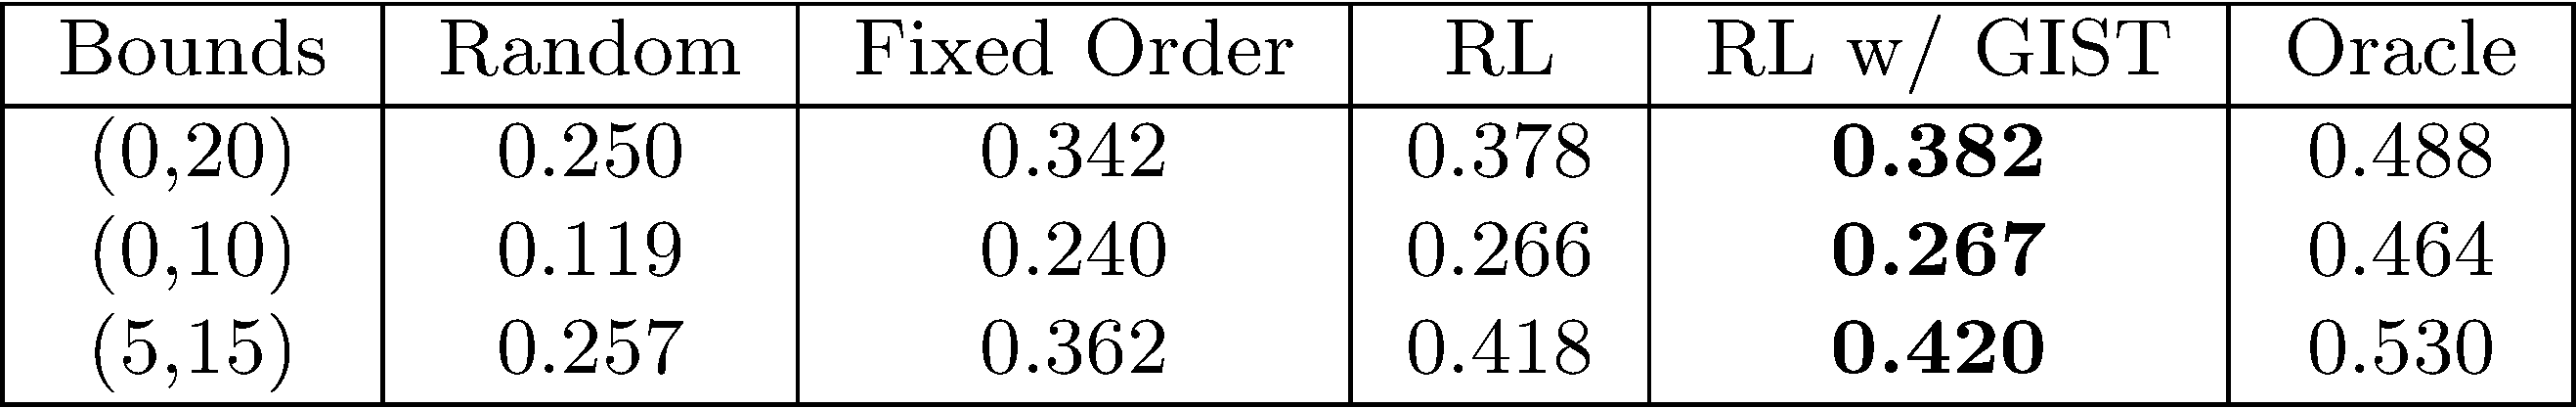
\includegraphics[width=15cm]{../../figures/table.pdf}\\\small{Areas under the AP vs. Time curve.}\end{center}
      }%
      \parbox{14cm}{\hfill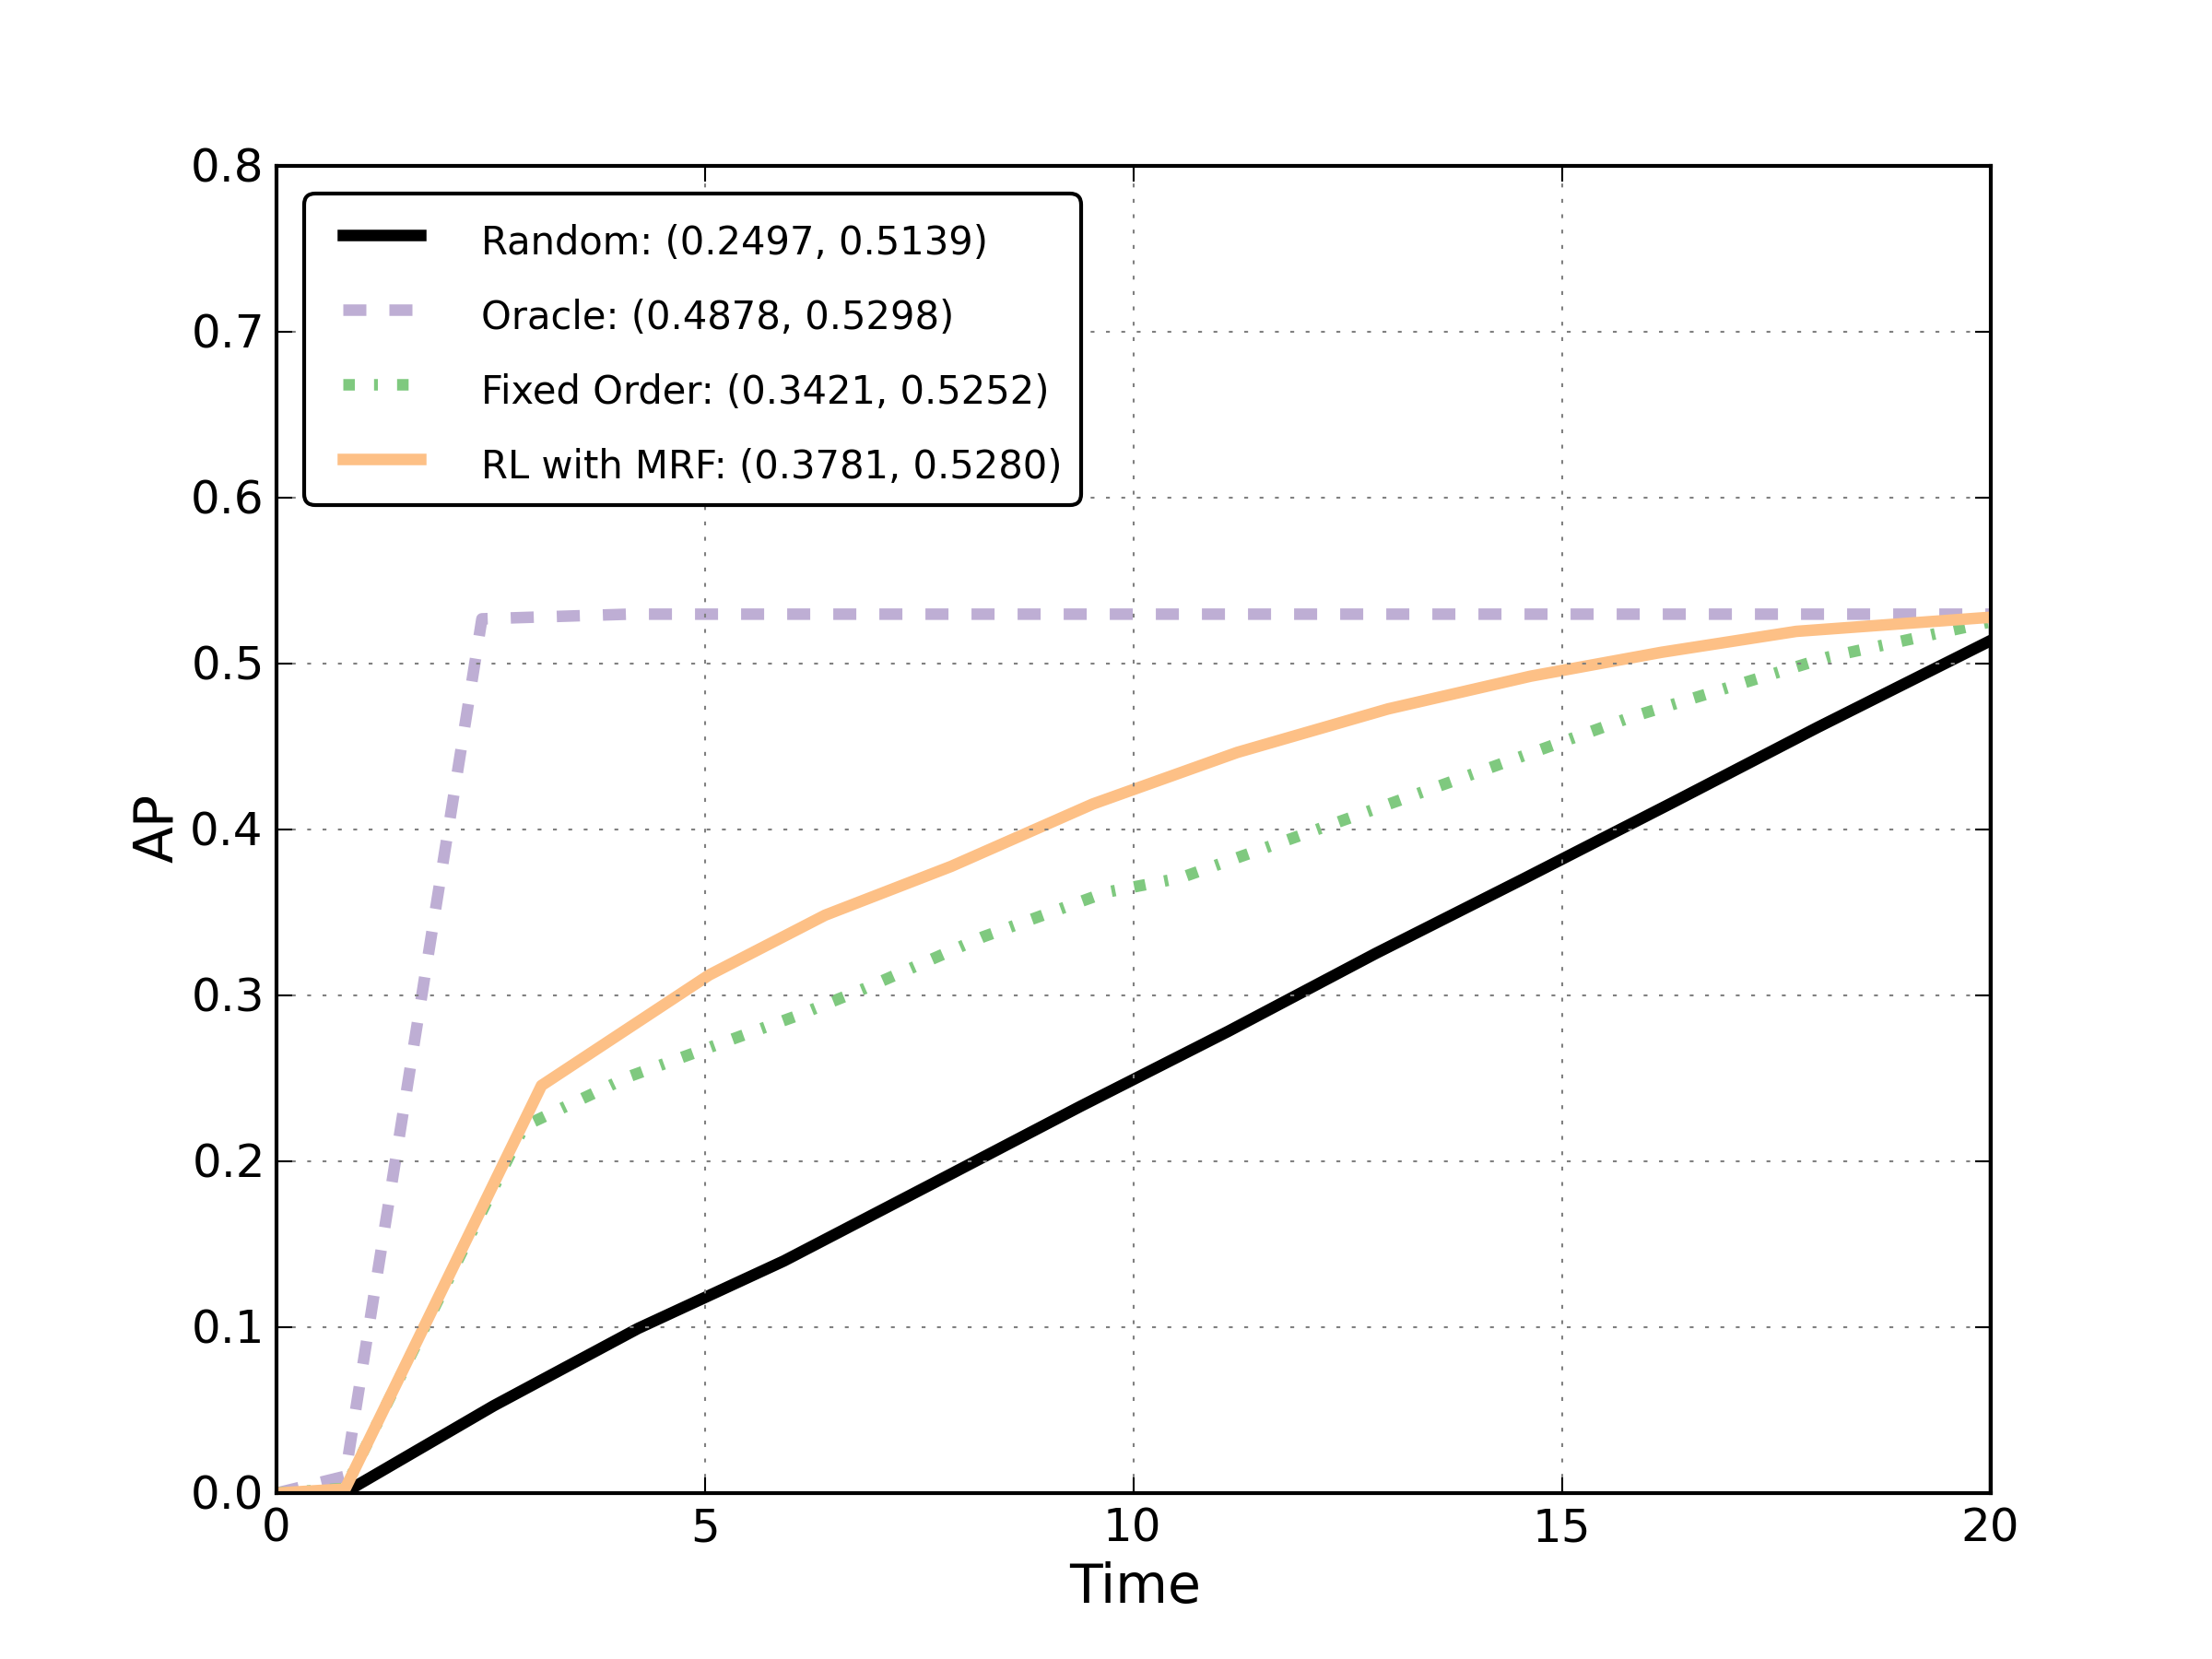
\includegraphics[width=13cm]{../../figures/final1.png}}
      \\

      \textbf{\textsc{Policy Trajectories}}
      \begin{center}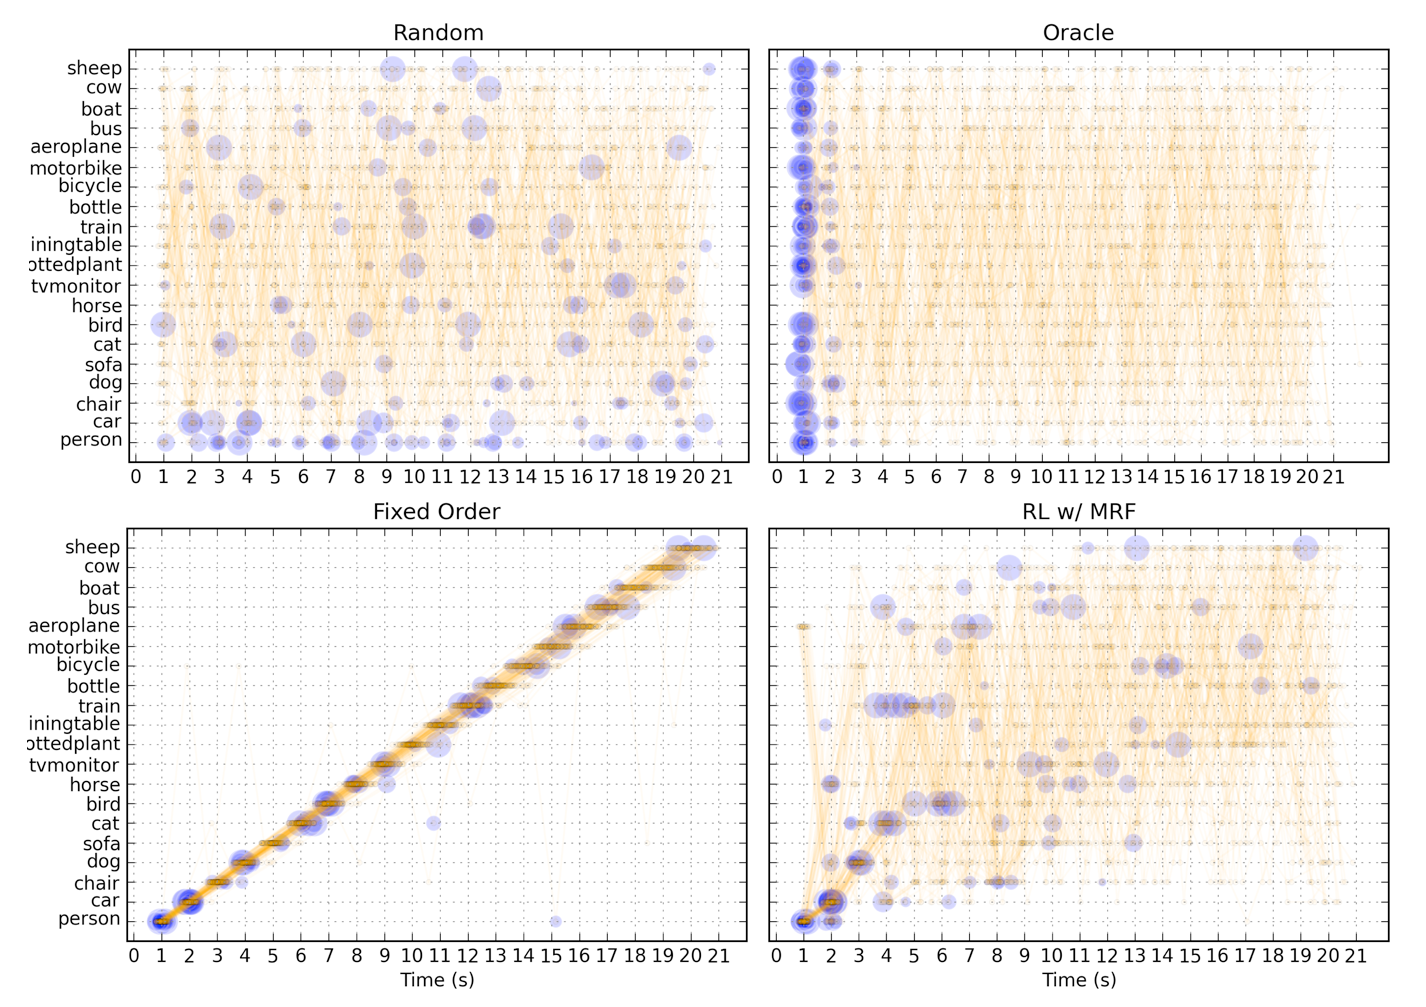
\includegraphics[height=13.6cm]{../../figures/trajectories.pdf}\end{center}

      Action selection traces are plotted over many episodes; the size of the circles correspond to the increase in AP obtained by the action. Our policy selects actions dynamically to maximize the rewards obtained early on.
    }; \addcenteredtitle{results}{5. Evaluation}

%%% Conclusion
    \path (results.south west) ++(0cm,-2cm) node(conclusion) [style=tbox,text width=28cm] {
      If execution is stopped with only half of the detectors deployed, we obtain at least $66\%$ better AP than a random ordering, and $14\%$ better than an intelligent baseline. On the timeliness measure, we obtain at least $11\%$ better performance.
      \vspace{7mm}
      
      Our method is easily extensible.\\
      Code is available at \url{http://sergeykarayev.com/work/timely/}.
      \vspace{7mm}

      \textbf{\textsc{Next Steps}}
      \begin{itemize}
        \item Define actions on regions of the image.
        \item Account for feature computation cost with multiple detector types.
      \end{itemize}
    }; \addcenteredtitle{conclusion}{6. Conclusion}
    
\end{tikzpicture}
\end{center}
\end{document}
